\def\rot{\rotatebox}
\newcolumntype{a}{>{\columncolor{gr1}}r}
\newcolumntype{b}{>{\columncolor{gr2}}r}
\newcolumntype{c}{>{\columncolor{gr3}}r}
\newcolumntype{d}{>{\columncolor{gr4}}r}
\begin{figure}[!htbp]
% \centering
% \arrayrulecolor[gray]{0.5}
% \resizebox{\linewidth}{!}{
% \begin{tabular}{@{}l|rrar|rrrb|rrrc|rrrd}
%             \rowcolor{white}& \multicolumn{4}{c|}{$0\leq Overlap<25$}       & \multicolumn{4}{c|}{$25\leq Overlap<50$}       & \multicolumn{4}{c|}{$50\leq Overlap<75$}       & \multicolumn{4}{c}{$75\leq Overlap\leq100$}      \bigstrut\\ \hline
%             & \rot{90}{ALVES} & \rot{90}{OLIVE} & \rot{90}{SHATW} & \rot{90}{XTREE} & \rot{90}{ALVES} & \rot{90}{OLIVE} & \rot{90}{SHATW} & \rot{90}{XTREE} & \rot{90}{ALVES} & \rot{90}{OLIVE} & \rot{90}{SHATW} & \rot{90}{XTREE} & \rot{90}{ALVES} & \rot{90}{OLIVE} & \rot{90}{SHATW} & \rot{90}{XTREE} \bigstrut\\ \hline
% ant-1      & 139   & 137   & 147   & 14    & 8     & 8     & 4     & 48    & 2     & 2     & 0     & 34    & 3     & 4     & 0     & 76    \bigstrut\\
% ant-2      & 252   & 249   & 263   & 15    & 11    & 10    & 0     & 76    & 1     & 2     & 0     & 45    & 0     & 0     & 0     & 153   \bigstrut\\ 
% ant-3      & 291   & 286   & 312   & 40    & 27    & 25    & 3     & 115   & 3     & 6     & 0     & 71    & 0     & 2     & 0     & 136   \bigstrut\\ \hline
% lucene-1   & 159   & 150   & 182   & 9     & 38    & 29    & 33    & 70    & 24    & 15    & 0     & 38    & 5     & 24    & 0     & 113   \bigstrut\\ \hline
% ivy-1      & \cellcolor{gr1}{39}    & \cellcolor{gr1}{39}    & 39    & 7     & 0     & 1     & 0     & 15    & 0     & 0     & 0     & 8     & 0     & 0     & 0     & 13    \bigstrut\\ \hline
% camel-1    & 437   & 431   & 513   & 119   & 33    & 34    & 0     & 115   & 34    & 16    & 0     & 70    & 23    & 42    & 0     & 248   \bigstrut\\ 
% camel-2    & 720   & 708   & 770   & 44    & 36    & 28    & 0     & 146   & 30    & 16    & 0     & 103   & 2     & 25    & 0     & 527   \bigstrut\\ \hline
% xerces-1   & 363   & 361   & 390   & 4     & 8     & 6     & 0     & 23    & 12    & 6     & 0     & 34    & 14    & 19    & 0     & 343   \bigstrut\\
% xerces-2   & 281   & 278   & 296   & 4     & 7     & 6     & 0     & 17    & 8     & 5     & 0     & 18    & 2     & 10    & 0     & 268   \bigstrut\\ \hline
% velocity-1 & 138   & 127   & 187   & 12    & 32    & 15    & 23    & 29    & 23    & 18    & 0     & 44    & 7     & 34    & 0     & 119   \bigstrut\\ \hline
% xalan-1    & 526   & 517   & 552   & 8     & 45    & 31    & 133   & 94    & 89    & 32    & 85    & 104   & 71    & 123   & 0     & 523   \bigstrut\\
% xalan-2    & 607   & 591   & 773   & 69    & 93    & 24    & 0     & 64    & 114   & 90    & 0     & 198   & 7     & 87    & 0     & 500   \bigstrut\\ \hline
% poi-1      & 268   & 265   & 271   & 3     & 3     & 2     & 13    & 7     & 11    & 2     & 0     & 8     & 1     & 13    & 0     & 265   \bigstrut\\
% poi-2      & 291   & 231   & 323   & 9     & 77    & 81    & 24    & 159   & 20    & 20    & 0     & 50    & 0     & 22    & 0     & 153   \bigstrut\\ \hline
% log4j-1    & 84    & 80    & 92    & 2     & 6     & 8     & 2     & 22    & 5     & 2     & 0     & 16    & 0     & 4     & 0     & 56    \bigstrut\\ \hline
% jedit-1    & 244   & 236   & 249   & 12    & 13    & 13    & 14    & 58    & 8     & 8     & 0     & 57    & 0     & 5     & 0     & 153   \bigstrut\\
% jedit-3    & 194   & 189   & 198   & 31    & 6     & 12    & 1     & 86    & 2     & 2     & 0     & 38    & 0     & 1     & 0     & 77    \bigstrut\\
% jedit-2    & 245   & 238   & 259   & 26    & 16    & 22    & 3     & 102   & 4     & 3     & 0     & 48    & 0     & 3     & 0     & 119   \bigstrut\\ 
% \end{tabular}}
\centering
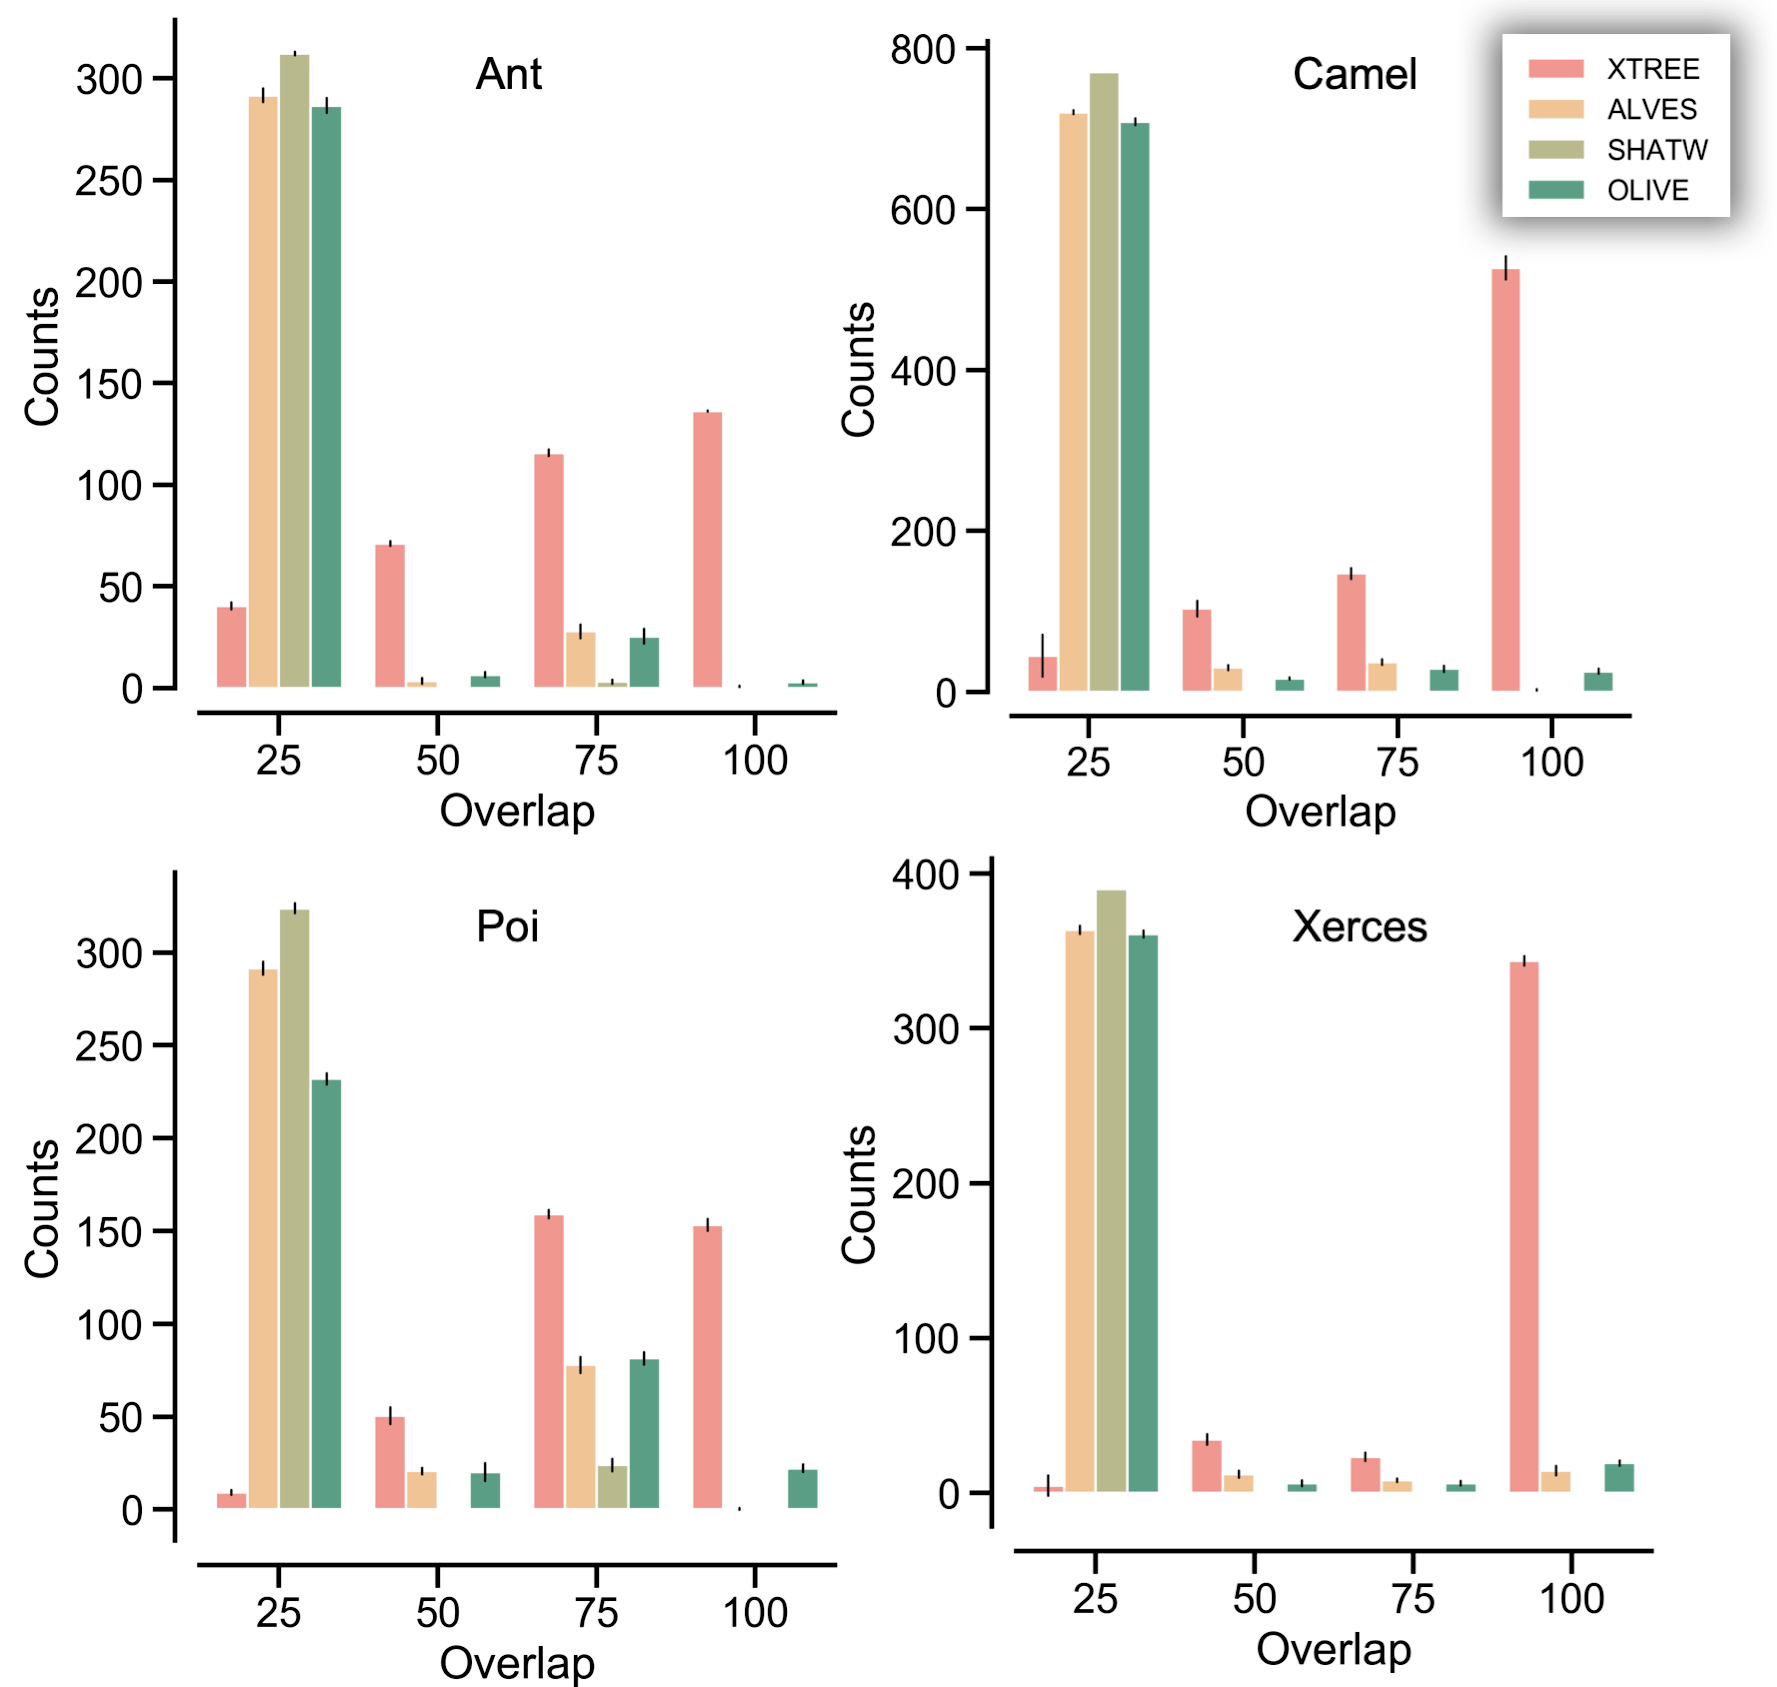
\includegraphics[width=0.75\linewidth]{rq1.png}
\caption{A count of number of test instances where the developer changes overlaps a planner recommendation. The overlaps (in the x-axis) are categorized into four ranges for every dataset (these are $0\leq~Overlap\leq25$, $26\leq~Overlap\leq50$, $51\leq~Overlap\leq75$, and $76\leq~Overlap\leq100$). For each of the overlap ranges, we count the the number of instances in the validation set where overlap between the planner's recommendation and the developers changes fell in that range. Note: \textit{Higher counts} for larger overlap is \textit{better}, e.g.,  $Count([75,100]) > Count([0,25))$ is considered better.}
\label{fig:results}
\end{figure}